\documentclass[12pt]{article}
\usepackage[margin=1in]{geometry}
\usepackage{graphicx}
\usepackage{float}
\usepackage{hyperref}
\usepackage{booktabs}
\usepackage{setspace}
\usepackage{amsmath}

\singlespacing
\begin{document}

\begin{titlepage}
    \vspace*{\fill}
    \begin{center}
        {\LARGE \bfseries Evaluating ML for EEG-Based\\Attention State Classification Under Budget Hardware Constraints\par}
        \vspace{1.5cm}
        {\Large Monir Fathalla\par}
        \vspace{1cm}
        {\large November 24, 2026\par}
    \end{center}
    \vspace*{\fill}
\end{titlepage}

\section{Introduction and Motivation}

I recently joined NeuraXtension, a student neuroscience club. The club is currently exploring projects involving brain-computer interfaces (BCIs), and one idea that came up was building an attention state classifier using electroencephalogram (EEG) data. This inspired the topic of my project: I wanted to investigate how well classical machine learning methods perform when constrained to the hardware specifications of the NeuroPawn, a budget consumer EEG headset with 8 channels (F3, Fz, F4, C3, C4, Pz, O1, O2) sampling at 125~Hz.

Most published EEG classification research uses medical-grade equipment with 32--64 electrodes at high sampling rates. The question I set out to answer is whether classical ML techniques can still distinguish between focused and unfocused mental states when limited to just 8 channels and a low sampling rate.

\section{Data Acquisition}

Finding suitable data proved to be one of the most difficult parts of the project. I initially searched Kaggle but found only heavily pre-processed, single-purpose datasets, and for ones that matched attention state the only one I found ended up being poorly structured and subpar in quality. I needed a competent dataset to build a realistic BCI pipeline from scratch.

I eventually found the XJTU-EEG MEMA (Multi-label EEG for Mental Attention states) dataset: 20 subjects, 12 trials each, totalling about 900 minutes of EEG in the trial files used here. However, the dataset was hosted exclusively on Baidu Pan, a Chinese cloud platform that is effectively inaccessible from North America without a local phone number. I found someone on a subreddit willing to download the data from Baidu and transfer it to me. I paid them \$16 in Ethereum. The full dataset was approximately 90~GB.

Each subject completed four rounds, and each round contains one trial of each state: attentive (\texttt{a}, about 5~minutes), neutral (\texttt{n}, 1~minute) and relaxed (\texttt{r}, about 5~minutes). Attentive trials are labelled \emph{focused} (1); neutral and relaxed trials are labelled \emph{unfocused} (0). About 46\% of the recorded time is therefore ``focused''.

\section{Data Cleaning and Preprocessing}

The raw MEMA data used here consists of comma-separated text files inside the \texttt{For\_graph} directory, one file per trial. Each file has 32 columns (one per electrode) recorded at 500~Hz.

My preprocessing script (\texttt{data\_processing.py}) treats every trial as one continuous signal:
\begin{enumerate}
    \item \textbf{Channel selection}: I keep only the 8 columns matching the NeuroPawn's electrode positions, located with the dataset's channel-to-electrode table (1-based channels 4, 3, 5, 14, 15, 23, 29 and 30). The table also identifies channel 18 as the CPz reference (a constant column) and channels 31--32 as horizontal eye-movement (EOG) channels.
    \item \textbf{Downsampling}: \texttt{scipy.signal.decimate} reduces the sampling rate from 500~Hz to 125~Hz, applying an anti-aliasing filter first.
    \item \textbf{Band-pass filtering}: a 4th-order Butterworth filter (second-order sections, zero-phase \texttt{sosfiltfilt}) keeps 0.5--45~Hz, removing slow drift and high-frequency noise.
\end{enumerate}
\textbf{Correction.} Earlier versions of this project (including the first version of this report) read columns that were assumed to be F3, Fz, F4, C3, C4, Pz, O1 and O2 but are actually Fz, F3, F4, Cz, C4, P3, T6 and O1. Five of the eight overlap, but C3, Pz and O2 were missing. The mapping was checked against the data: every electrode's signal correlates most strongly with its physical neighbours (for example F3 with FC3, T4 with TP8, O1 with Oz). All results in this report use the corrected columns, and Section~\ref{sec:channels} compares both sets directly.

Each cleaned trial is stored as a single float32 array together with its metadata (subject, round 1--4, state \texttt{a}/\texttt{n}/\texttt{r}, trial id). Files are processed in sorted order so the output is reproducible. Windowing is deferred to the feature step so that the window length can be tuned.

\section{Windowing and Feature Extraction}

\subsection{Windows}

\texttt{feature\_extraction.py} cuts each trial into windows with 50\% overlap. Overlap increases the number of windows, but neighbouring windows share half of their samples, so it does not add new information or ``double'' the usable data; it mainly gives a finer time grid for the smoothing step described later. Windows never cross trial boundaries.

I compared 1~s, 2~s and 4~s windows by cross-validation on rounds 1--3 only (round 4 was never used), with a fixed reference pipeline (per-subject z-scoring, LightGBM, 5~s smoothing). Table~\ref{tab:windows} shows that longer windows were better in both scenarios, so 4~s windows (2~s step) are used from here on.

\begin{table}[H]
\centering
\caption{Window length comparison: cross-validated accuracy on rounds 1--3 (LightGBM reference pipeline). Subject-dependent CV holds out one training round per subject; cross-subject CV is a 5-fold GroupKFold by subject.}
\label{tab:windows}
\begin{tabular}{lcccccc}
\toprule
Window & Step & Windows & \multicolumn{2}{c}{Subject-dependent} & \multicolumn{2}{c}{Cross-subject} \\
 & & & Raw & Smoothed & Raw & Smoothed \\
\midrule
1 s & 0.5 s & 108{,}097 & 60.9\% & 64.7\% & 59.6\% & 66.2\% \\
2 s & 1 s & 53{,}578 & 62.1\% & 65.2\% & 61.0\% & 67.1\% \\
4 s & 2 s & 26{,}639 & \textbf{64.8\%} & \textbf{66.3\%} & \textbf{65.3\%} & \textbf{69.3\%} \\
\bottomrule
\end{tabular}
\end{table}

\subsection{Features}

From each window I extract 11 features per channel, 88 in total:
\begin{itemize}
    \item \textbf{Log band powers} (5): power in Delta (0.5--4~Hz), Theta (4--8~Hz), Alpha (8--13~Hz), Beta (13--30~Hz) and Gamma (30--45~Hz), integrated from a Welch power spectrum (1~s segments for 2--4~s windows) and log-transformed to compress their right-skewed distributions.
    \item \textbf{Log band ratios} (3): Alpha/Beta, Theta/Beta and Theta/Alpha, which prior literature has linked to attention and ADHD markers. Taking logs makes them differences of log powers; tree models are unaffected, while linear models see better-behaved inputs.
    \item \textbf{Statistical features} (3): log standard deviation, skewness and kurtosis of the time-domain signal.
\end{itemize}
The window mean used in the previous version was dropped: after the 0.5~Hz high-pass it is essentially zero. The feature file stores only these base features plus each window's subject, trial id, round and label; feature selection now happens inside the model pipeline (Section~\ref{sec:selection}).

\section{Experimental Design}

\subsection{Evaluation scenarios}

\begin{itemize}
    \item \textbf{Subject-dependent}: train on rounds 1--3, test on round 4 of the same subject. This simulates a device calibrated with a few labelled sessions from its user.
    \item \textbf{Cross-subject}: leave-one-subject-out. Train on 19 subjects and test on all 12 trials of the held-out subject. This simulates a new user with no labelled calibration data.
\end{itemize}

\subsection{Per-subject normalization}

EEG amplitude and spectral baselines differ strongly between people. Every feature is therefore z-scored per subject using that subject's own mean and standard deviation. In the subject-dependent scenario the statistics come from the training rounds (z-scoring round 4 with its own statistics gave no gain in an earlier experiment). In the cross-subject scenario every subject, including the held-out one, is normalized with its own statistics. For the held-out subject this uses its recordings but never its labels, so it acts as an unlabeled calibration step.

\subsection{Feature selection, models and model selection}
\label{sec:selection}

Feature selection is the first step of an sklearn \texttt{Pipeline}, so it is fit on training folds only:
\begin{enumerate}
    \item \textbf{None}: all 88 features.
    \item \textbf{ANOVA}: the 30 features with the highest F-statistic. (The old $p \le 0.05$ rule keeps almost every feature when tens of thousands of windows are pooled, so a fixed count is used.)
    \item \textbf{Feature importance (FI)}: features with above-average random forest importance.
    \item \textbf{Linear correlation (LCC)}: features whose absolute Pearson correlation with the label is above the mean absolute correlation.
    \item \textbf{PCA}: standardized features projected onto the components that explain 95\% of the variance.
\end{enumerate}
The classifiers are shrinkage LDA, logistic regression ($C \in \{0.01, 1\}$), KNN ($k \in \{15, 51\}$), random forest (200 trees) and LightGBM (two settings: 200 trees with 15 leaves, and 500 trees with 31 leaves). \texttt{class\_weight='balanced'} (or equal priors for LDA) is used wherever supported. In addition, three soft-voting ensembles average the predicted probabilities of their members: LDA + LightGBM; logistic regression + random forest + LightGBM; and all four of LDA, logistic regression, random forest and LightGBM (members use the first hyperparameter setting listed above). This gives $5 \times 11 = 55$ candidate configurations. The single decision tree from the previous version was replaced by LDA and logistic regression, which are standard linear baselines for EEG. SVMs were not included: kernel SVMs scale poorly to the tens of thousands of windows in the cross-subject training sets.

The configuration is chosen by grouped cross-validation on training data only; the test data never selects a model:
\begin{itemize}
    \item \textbf{Subject-dependent}: leave-one-round-out over rounds 1--3 (3 folds). Besides the 55 configurations, I also compare two training pools: \emph{own} (one model per subject, trained only on that subject's data) and \emph{pooled} (one model trained on the training rounds of all 20 subjects, each z-scored with its own statistics). Both pools only ever see rounds 1--3. The candidate with the best mean CV accuracy across subjects is then refit on rounds 1--3 and tested on round 4.
    \item \textbf{Cross-subject}: nested cross-validation. For each of the 20 held-out subjects, a 4-fold GroupKFold over the remaining 19 subjects ranks the 55 configurations; the winner is refit on all 19 subjects and tested on the held-out subject. The selected configuration may differ between outer folds.
\end{itemize}
The selection score is smoothed accuracy (next section), which is the output the system would actually show.

\subsection{Causal smoothing}

A person's attention state persists for many seconds, while single 4~s windows are noisy. The predicted probability of ``focused'' is therefore averaged over the current and previous windows covering the past 5~s (3 windows with a 2~s step), within a trial only. The average only uses past windows, so it could run online; the first windows of a trial average over whatever history exists. The 5~s horizon was fixed in advance and was not tuned on test data. I report both raw-window and smoothed metrics.

\subsection{Metrics}

For each test subject I compute accuracy, balanced accuracy and macro F1, and report the mean $\pm$ standard deviation across the 20 subjects. The baseline always predicts the majority class of the training data.

\section{Results}

\subsection{Selected configurations}

Figure~\ref{fig:cv} shows the cross-validated accuracy of every model and feature-selection method; these are the scores the configurations were chosen by. The differences between the best candidates are small (well under one percentage point), while KNN is clearly weaker.

\begin{itemize}
    \item \textbf{Subject-dependent}: shrinkage LDA on all 88 features, trained per subject (\emph{own} pool), CV accuracy 69.8\%. The best pooled candidate (LightGBM trained on all subjects' rounds 1--3) reached 69.5\% and the best ensemble 69.3\%, so neither pooling nor combining models helped here.
    \item \textbf{Cross-subject}: 19 of the 20 outer folds chose an ensemble on all 88 features (logistic regression + random forest + LightGBM in 17 folds, all four models in 2); one fold chose a random forest. In the inner CV, the best ensemble scored 67.6\% against 67.2\% for the best single model.
\end{itemize}

\begin{figure}[H]
    \centering
    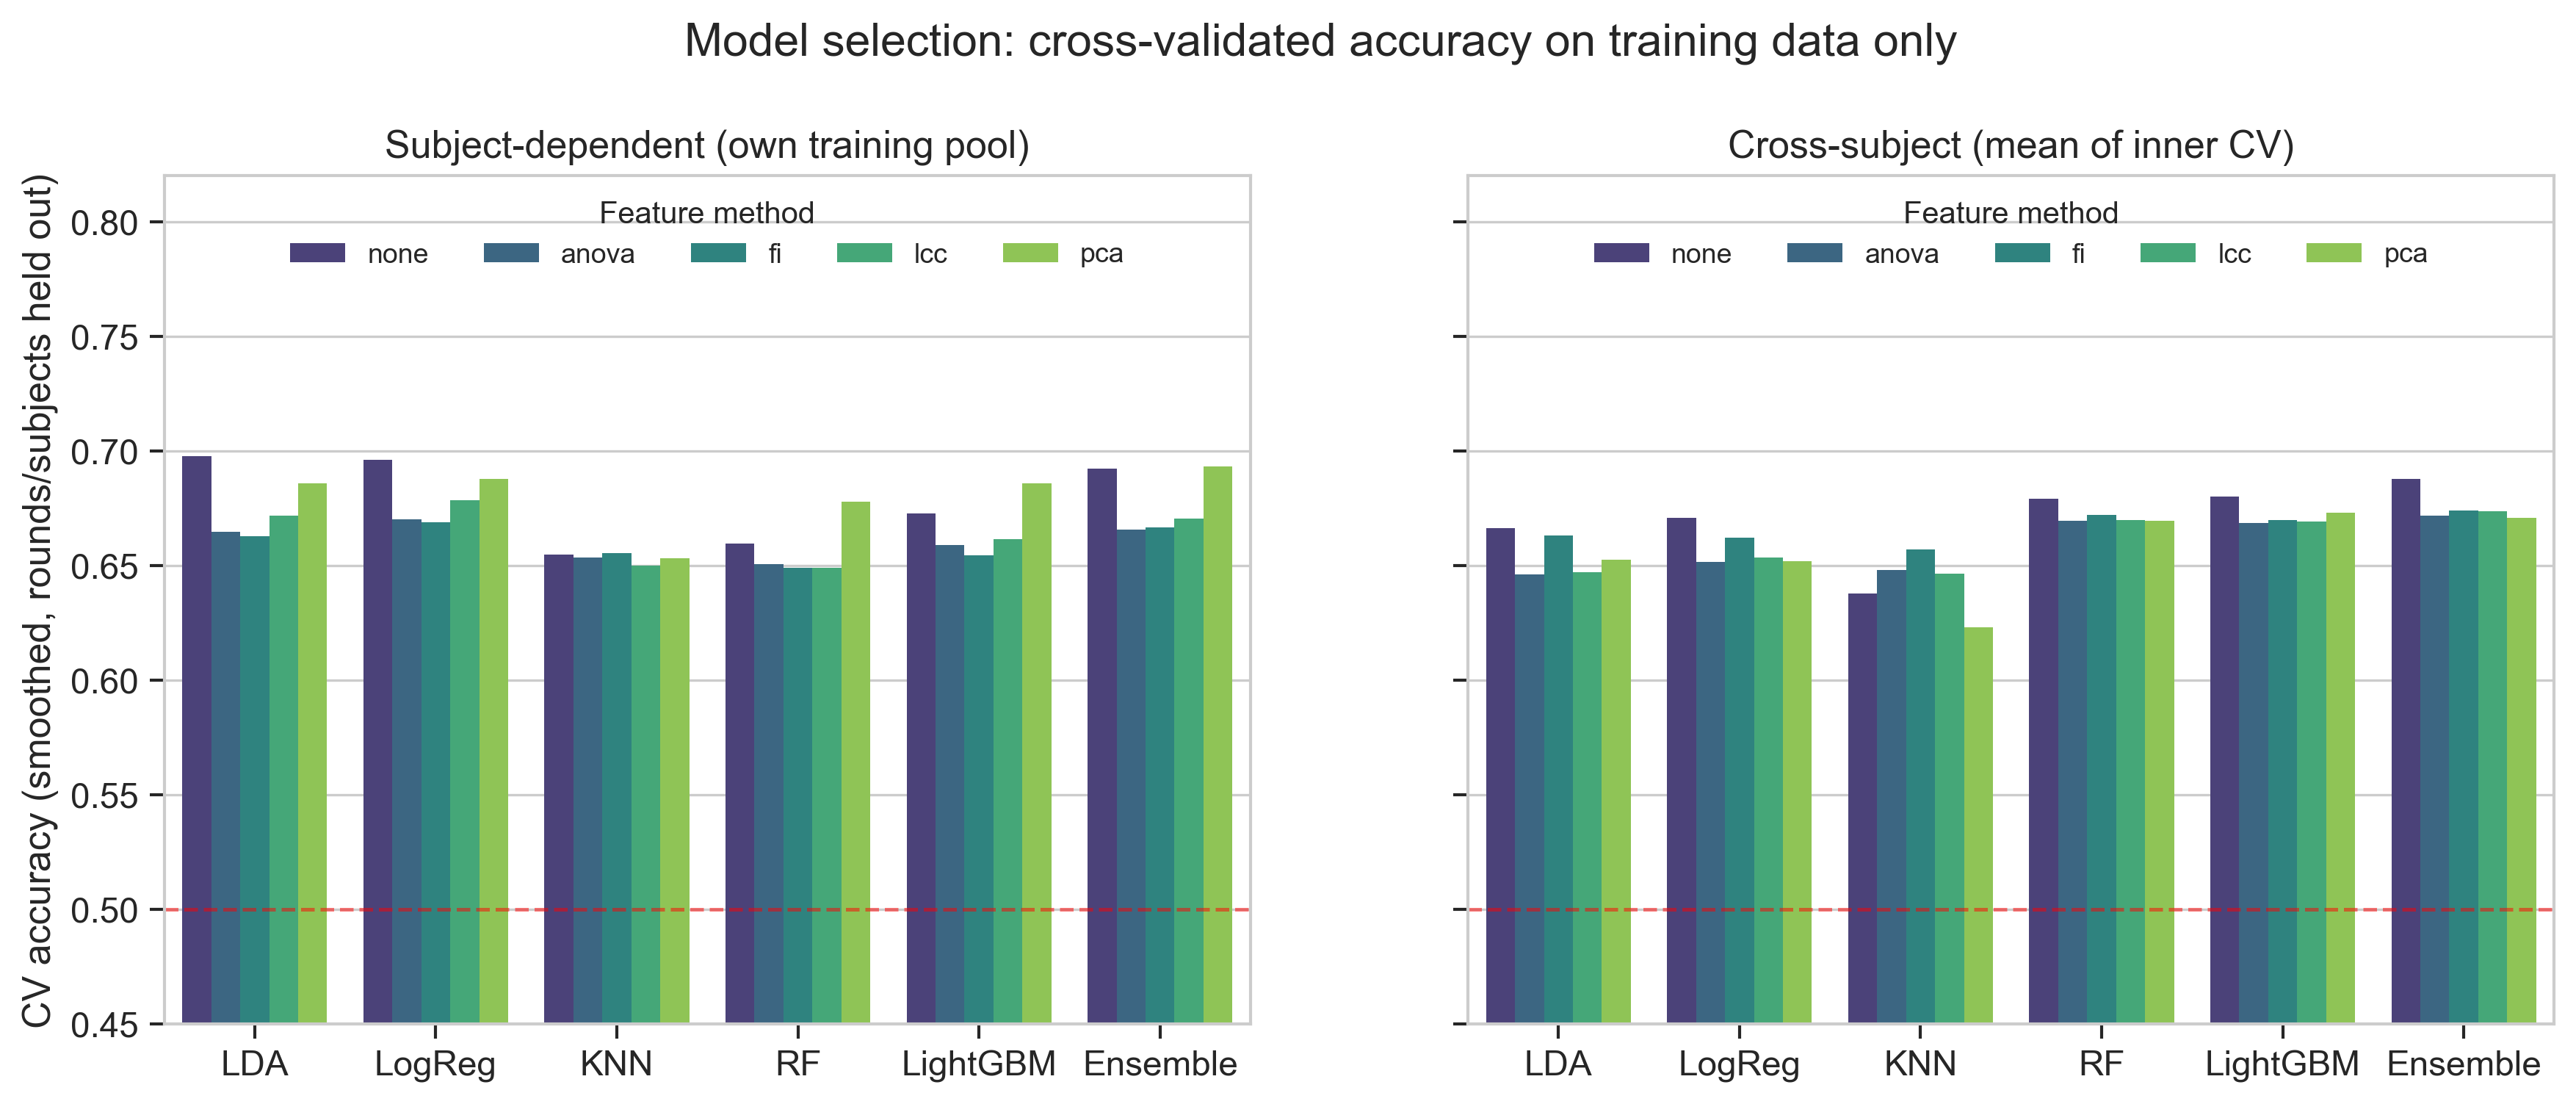
\includegraphics[width=\textwidth]{results/figures/cv_model_comparison.png}
    \caption{Cross-validated (smoothed) accuracy of each model and feature method on training data only, using the best hyperparameter setting of each pair. Left: leave-one-round-out over rounds 1--3. Right: inner GroupKFold scores averaged over the 20 outer folds.}
    \label{fig:cv}
\end{figure}

\subsection{Test results}

Table~\ref{tab:results} reports the test performance of the selected pipelines. The majority-class baseline is 55.1\% (subject-dependent) and 52.4\% (cross-subject), so the classes are roughly balanced, and accuracy, balanced accuracy and macro F1 agree closely.

\begin{table}[H]
\centering
\caption{Test results with the NeuroPawn electrodes, mean $\pm$ standard deviation across the 20 subjects. ``Raw'' scores single 4~s windows; ``smoothed'' averages the predicted probability over the past 5~s within the trial.}
\label{tab:results}
\begin{tabular}{llccc}
\toprule
Scenario & Output & Accuracy & Balanced acc. & Macro F1 \\
\midrule
Subject-dependent & Baseline & 55.1\% & 50.0\% & -- \\
 & Raw window & 69.0 $\pm$ 11.7\% & 69.9 $\pm$ 11.2\% & 0.680 $\pm$ 0.126 \\
 & Smoothed & \textbf{70.6 $\pm$ 12.9\%} & \textbf{71.7 $\pm$ 12.5\%} & \textbf{0.694 $\pm$ 0.141} \\
\midrule
Cross-subject & Baseline & 52.4\% & 50.0\% & -- \\
 & Raw window & 65.3 $\pm$ 7.2\% & 65.2 $\pm$ 7.3\% & 0.652 $\pm$ 0.073 \\
 & Smoothed & \textbf{69.4 $\pm$ 8.8\%} & \textbf{69.3 $\pm$ 8.8\%} & \textbf{0.693 $\pm$ 0.089} \\
\bottomrule
\end{tabular}
\end{table}

The previous version of this project reported 66.9\% (subject-dependent) and 58.0\% (cross-subject). Those numbers came from the mislabelled electrode set and from picking the best of 20 model/feature combinations by test accuracy, so they are not directly comparable. The new numbers use the correct electrodes and configurations chosen without looking at the test data. They are 3.7 points higher subject-dependent and 11.4 points higher cross-subject after smoothing. With the mislabelled set, the same new pipeline reached 77.2\% and 73.7\%. The difference comes from the electrodes, not the method (Section~\ref{sec:channels}).

\begin{figure}[H]
    \centering
    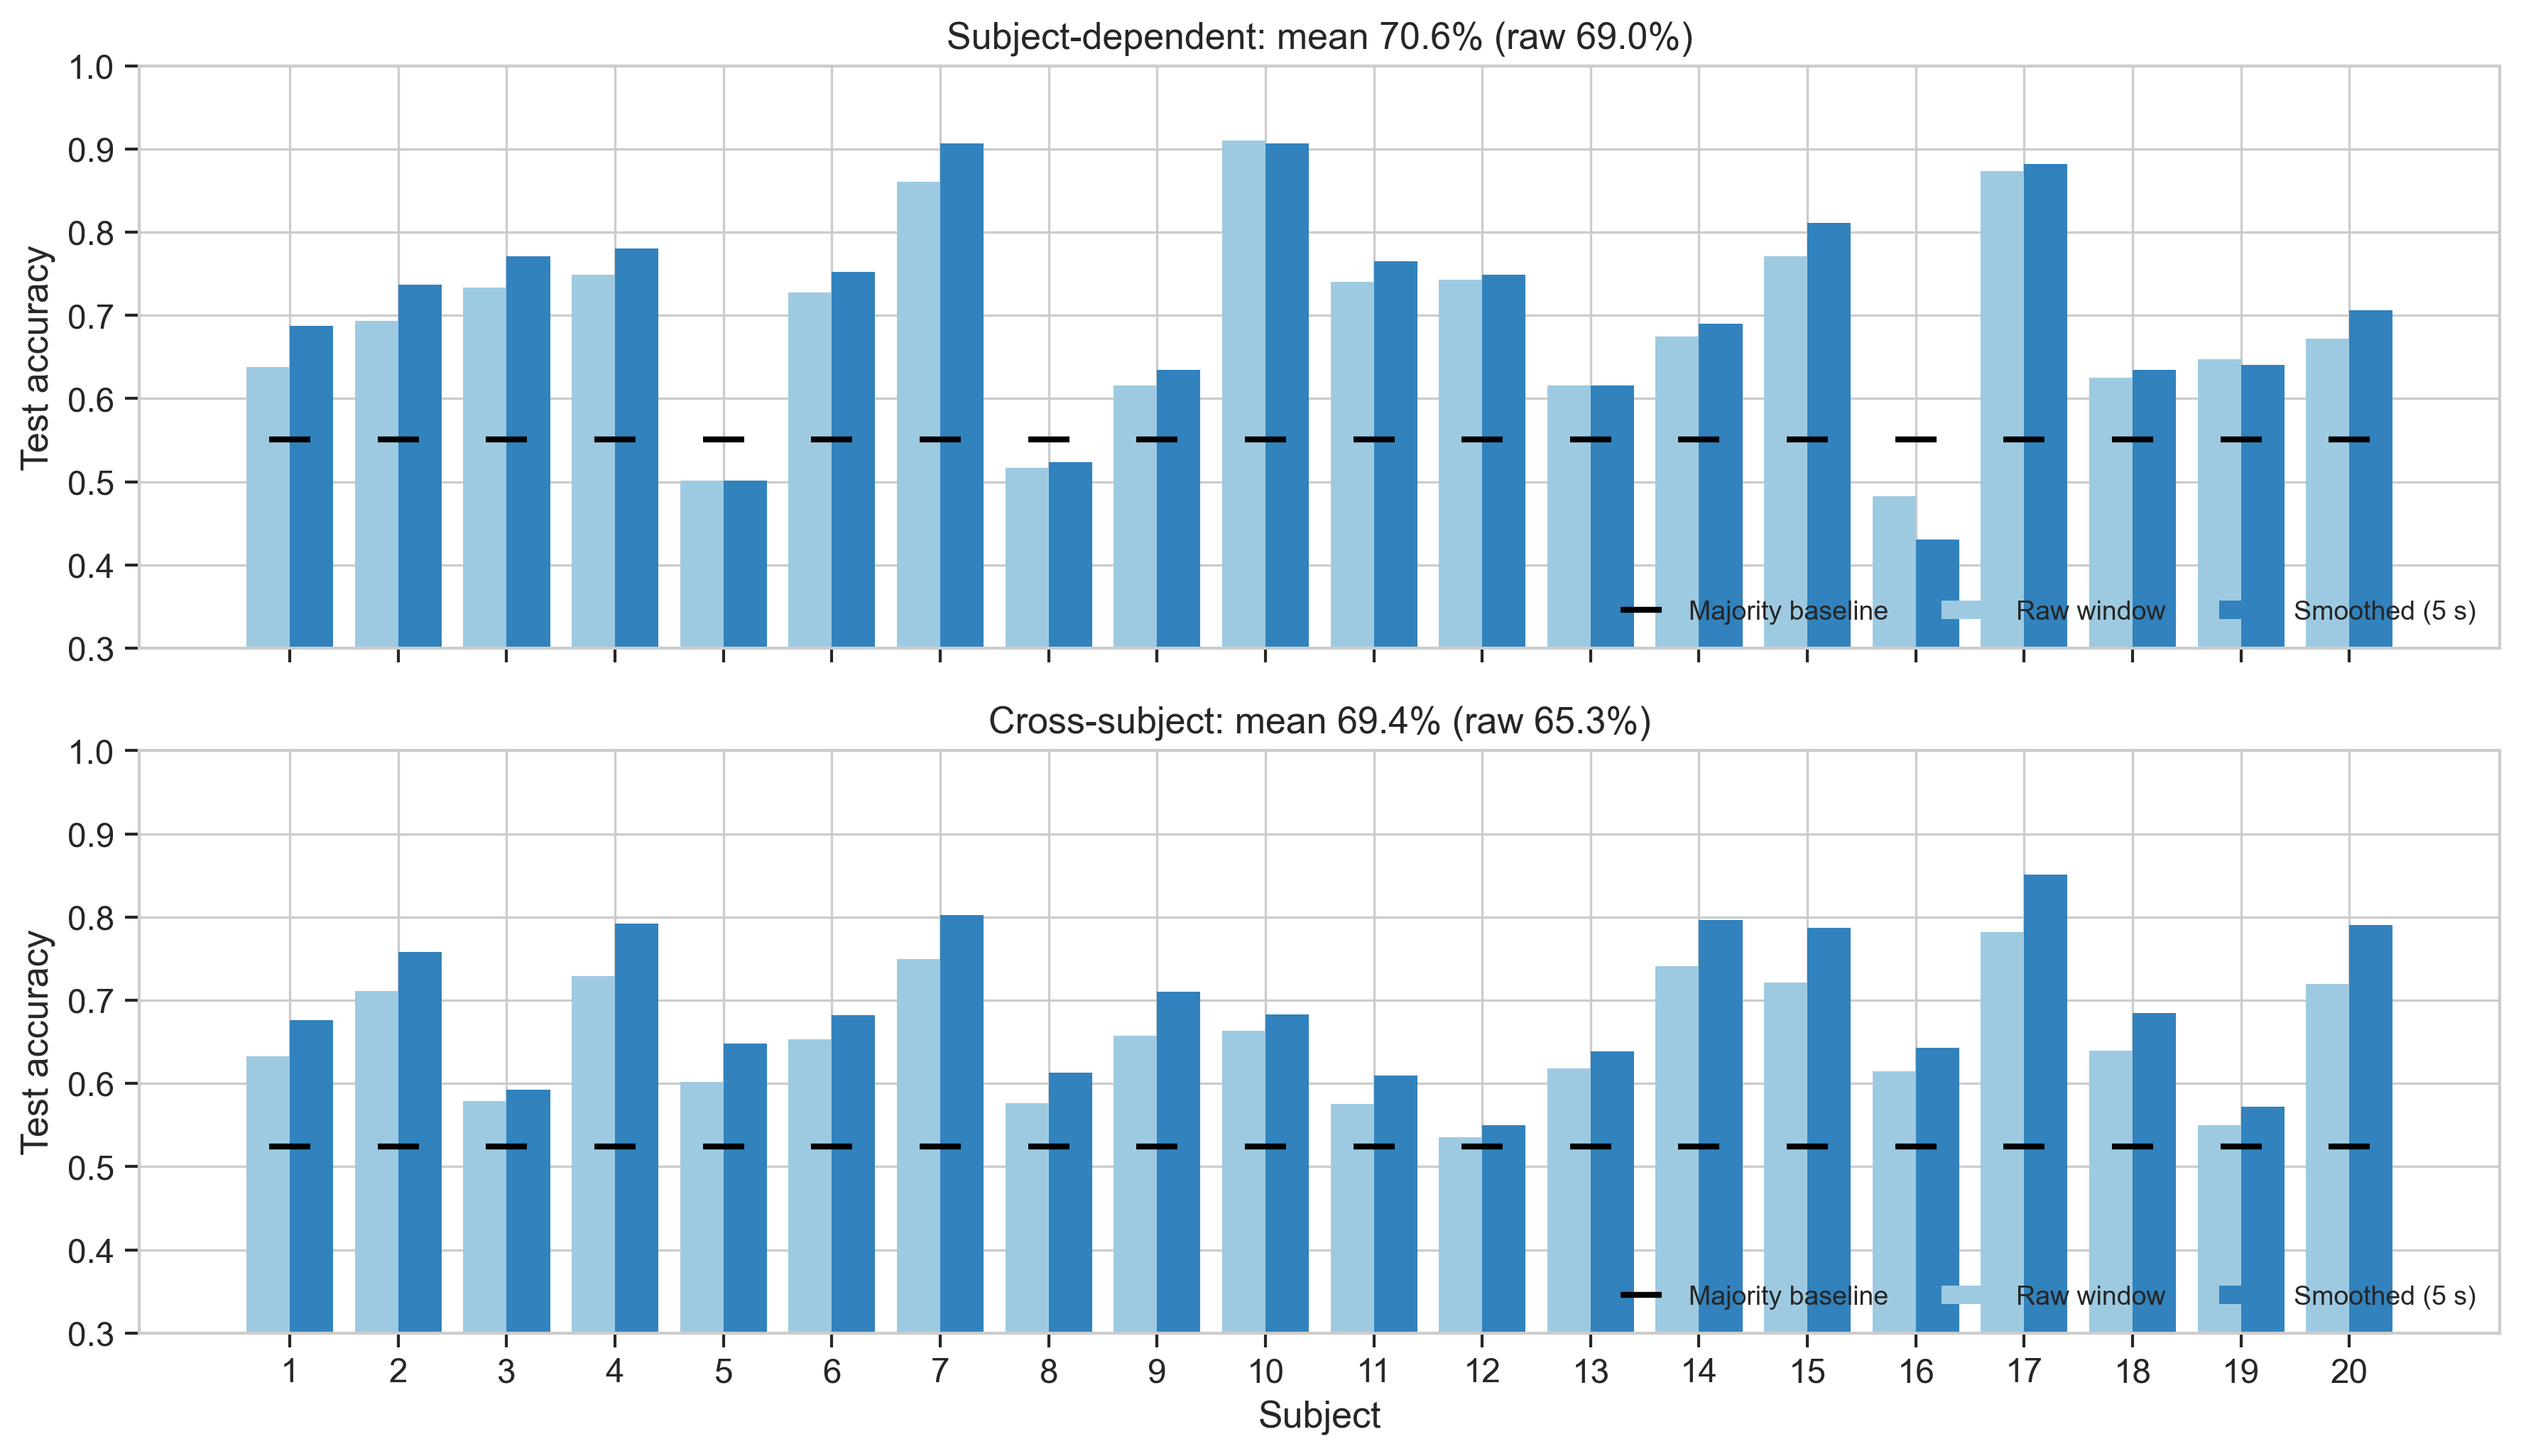
\includegraphics[width=\textwidth]{results/figures/per_subject.png}
    \caption{Test accuracy per subject. Black marks show the majority-class baseline.}
    \label{fig:subjects}
\end{figure}

Performance varies a lot between people (Figure~\ref{fig:subjects}): smoothed accuracy ranges from 43\% to 91\% in the subject-dependent scenario and from 55\% to 85\% across subjects. All 20 held-out subjects are above the cross-subject baseline. In the subject-dependent scenario, subjects 5, 8 and 16 are at or below the baseline.

\begin{figure}[H]
    \centering
    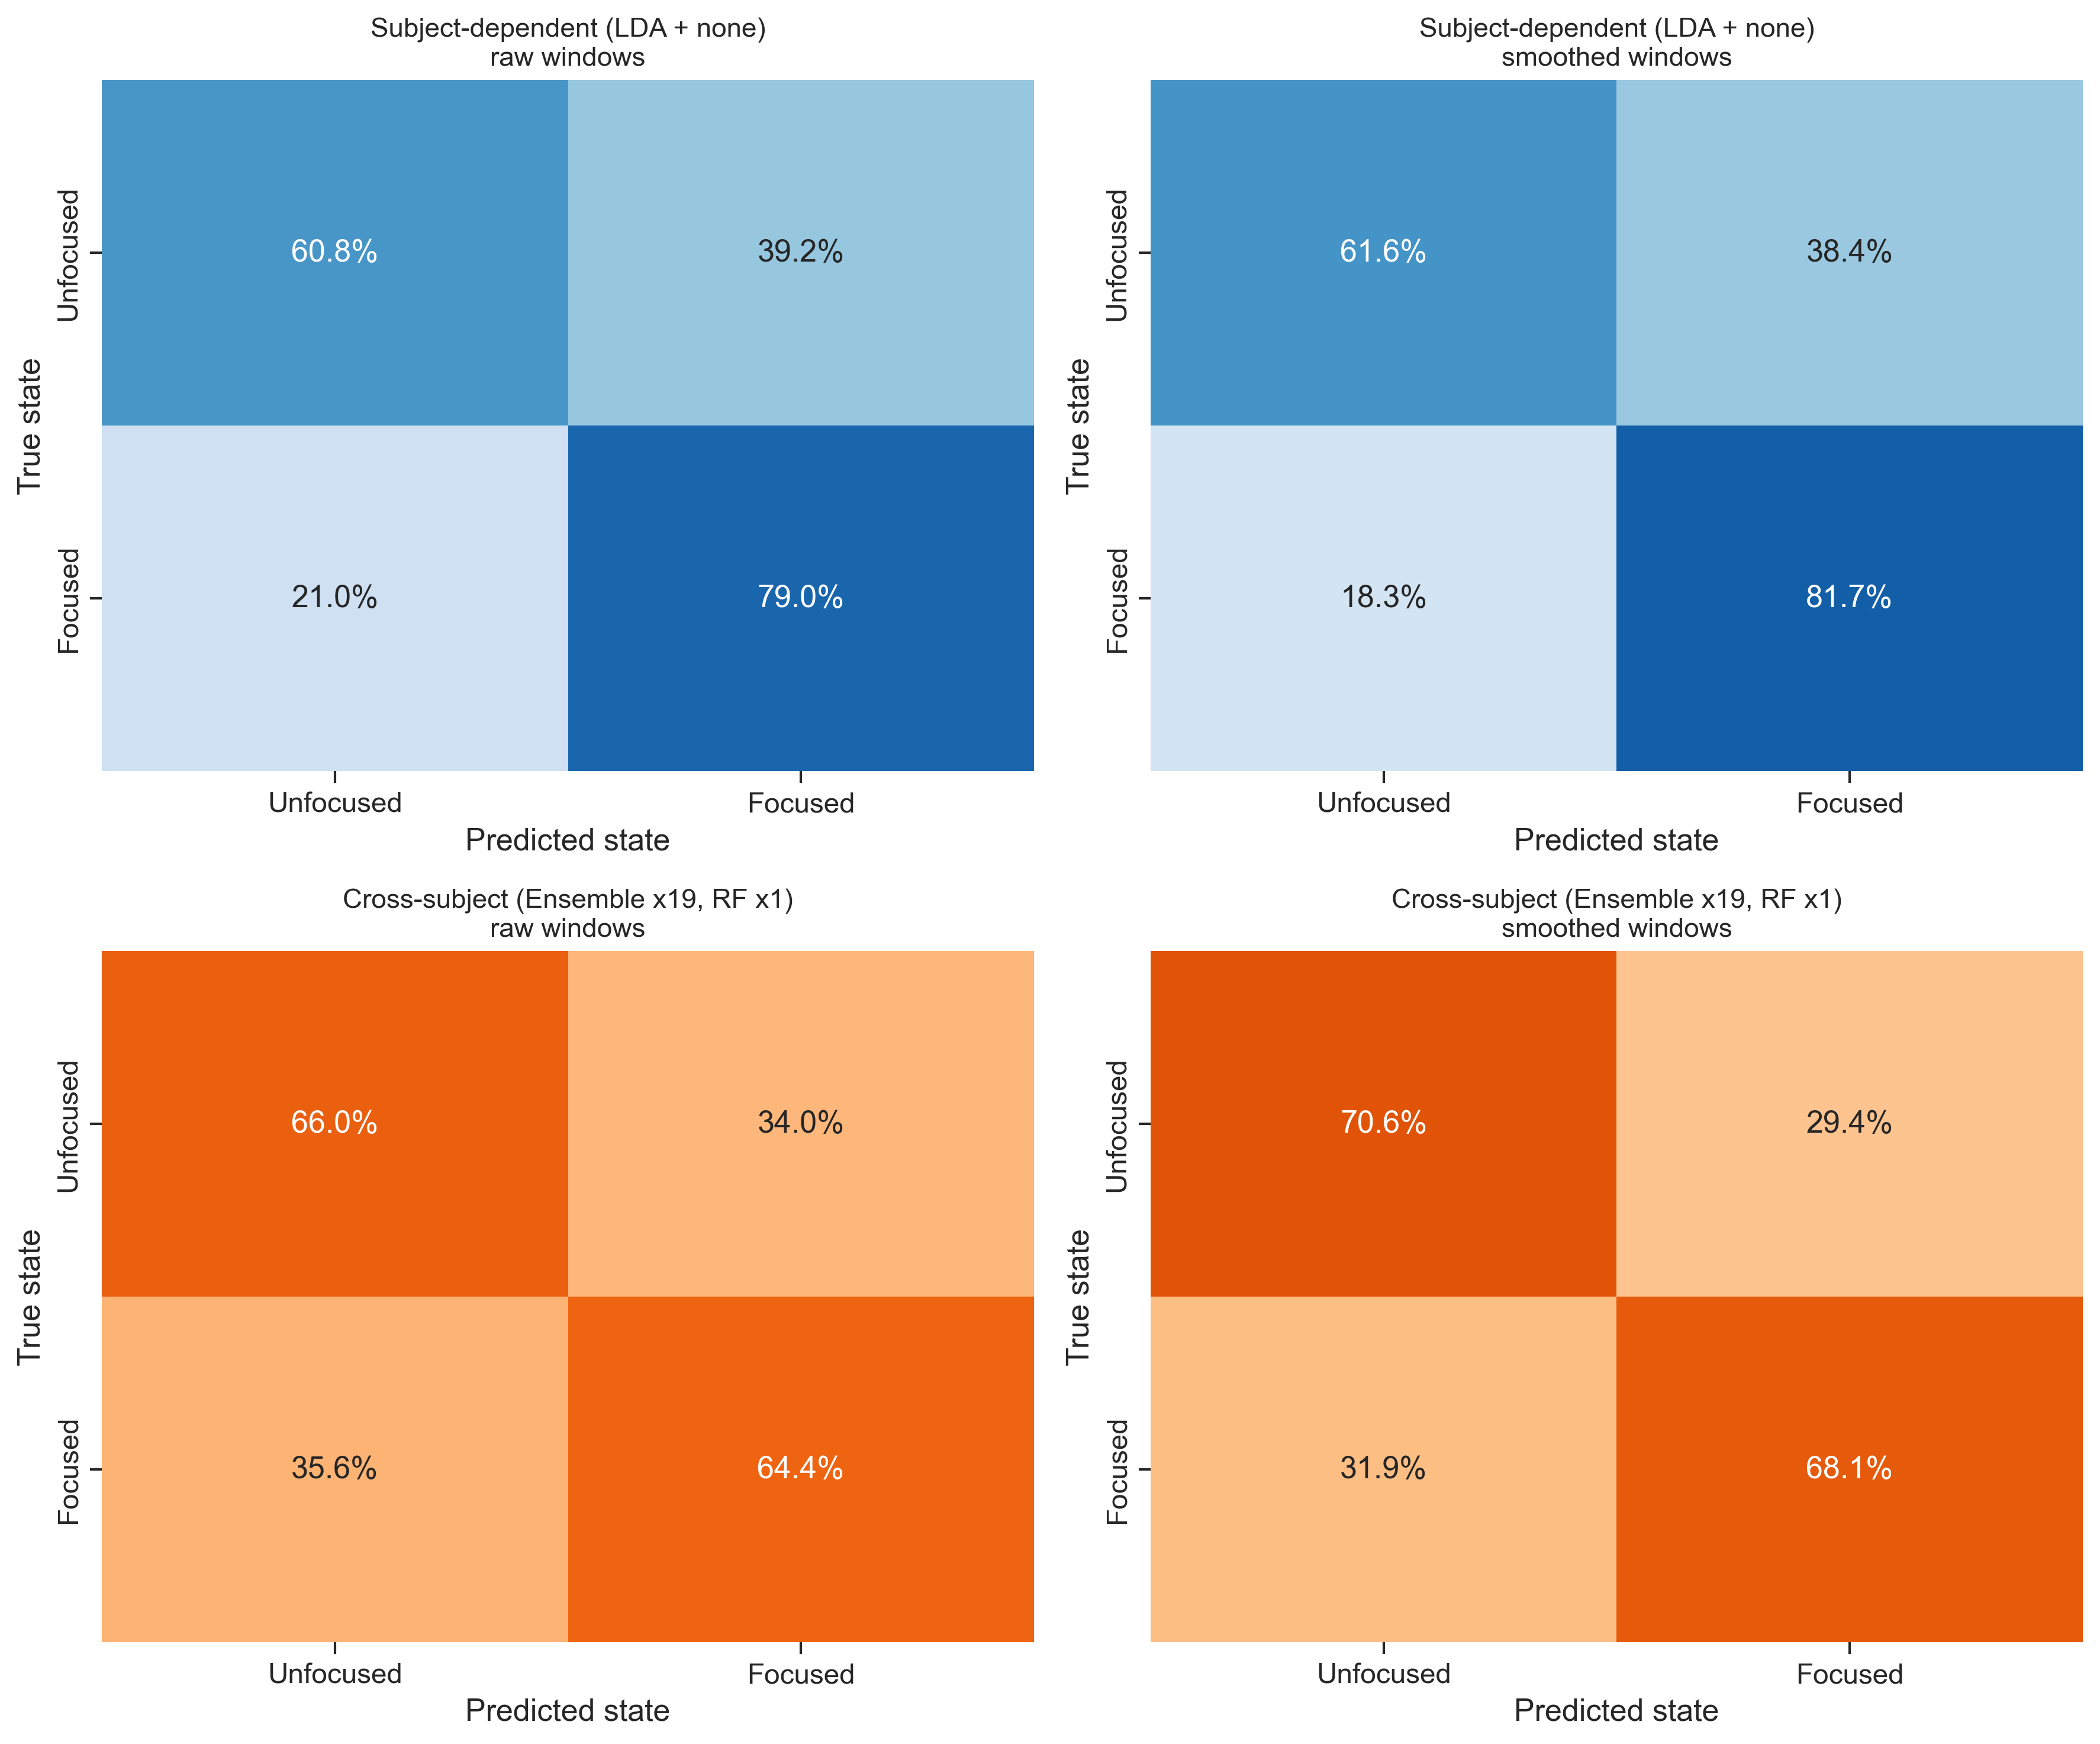
\includegraphics[width=0.85\textwidth]{results/figures/confusion_matrix.png}
    \caption{Confusion matrices aggregated over all 20 subjects for the selected pipelines (rows normalized), raw and smoothed.}
    \label{fig:confusion}
\end{figure}

\subsection{Why accuracy differs between subjects}

To understand the spread, \texttt{subject\_diagnostics.py} computes a few descriptive measures per subject (Figure~\ref{fig:diagnostics}). With 20 subjects, the correlations below are indicative rather than conclusive.

\begin{itemize}
    \item \textbf{The common pattern.} Across subjects, the most consistent difference is \emph{more} theta power over the occipital electrodes (O1, O2) during the attentive task, together with higher theta/alpha and theta/beta ratios at O1, O2, C3 and F3. The direction is the same in 80--90\% of subjects.
    \item \textbf{Signal strength.} How different the two states look for a person (mean $|d|$ of their 10 most different features) tracks test accuracy closely (Spearman $\rho = 0.79$ subject-dependent, $0.64$ cross-subject). This measure uses all of the person's labels, so it describes rather than explains: for low scorers such as subjects 5, 8, 16 and 19, focused and unfocused recordings simply look alike at these electrodes.
    \item \textbf{Stability across rounds.} Whether a person's focused-vs-unfocused pattern in round~4 matches rounds 1--3 strongly predicts subject-dependent accuracy ($\rho = 0.71$, $p < 0.001$). For subjects 9 and 16 the pattern even reverses (correlation $-0.11$ and $-0.08$). Their own model then fails (63\% and 43\%), while the population model does better (71\% and 64\%). Subject~5's round-4 features moved furthest from rounds 1--3 (0.74 standard deviations), and their own model is at chance on round~4 (50\%) but not on the other rounds. Subject~15 is only readable later in the session: about 45\% when round 1 or 2 is held out, over 80\% for rounds 3--4.
    \item \textbf{Typicality.} How closely a person's pattern matches the average of the other 19 subjects relates to cross-subject accuracy ($\rho = 0.43$, $p = 0.06$) but not to subject-dependent accuracy. Subjects 3, 10, 11 and 12 have unusual patterns and reach 75--91\% with their own model but only 55--68\% with a model trained on others.
    \item \textbf{Noise.} The rate of large-amplitude bursts, the share of muscle-band power and the share of slow frontal power showed no clear association with accuracy ($|\rho| \le 0.33$, all $p > 0.15$).
\end{itemize}

\begin{figure}[H]
    \centering
    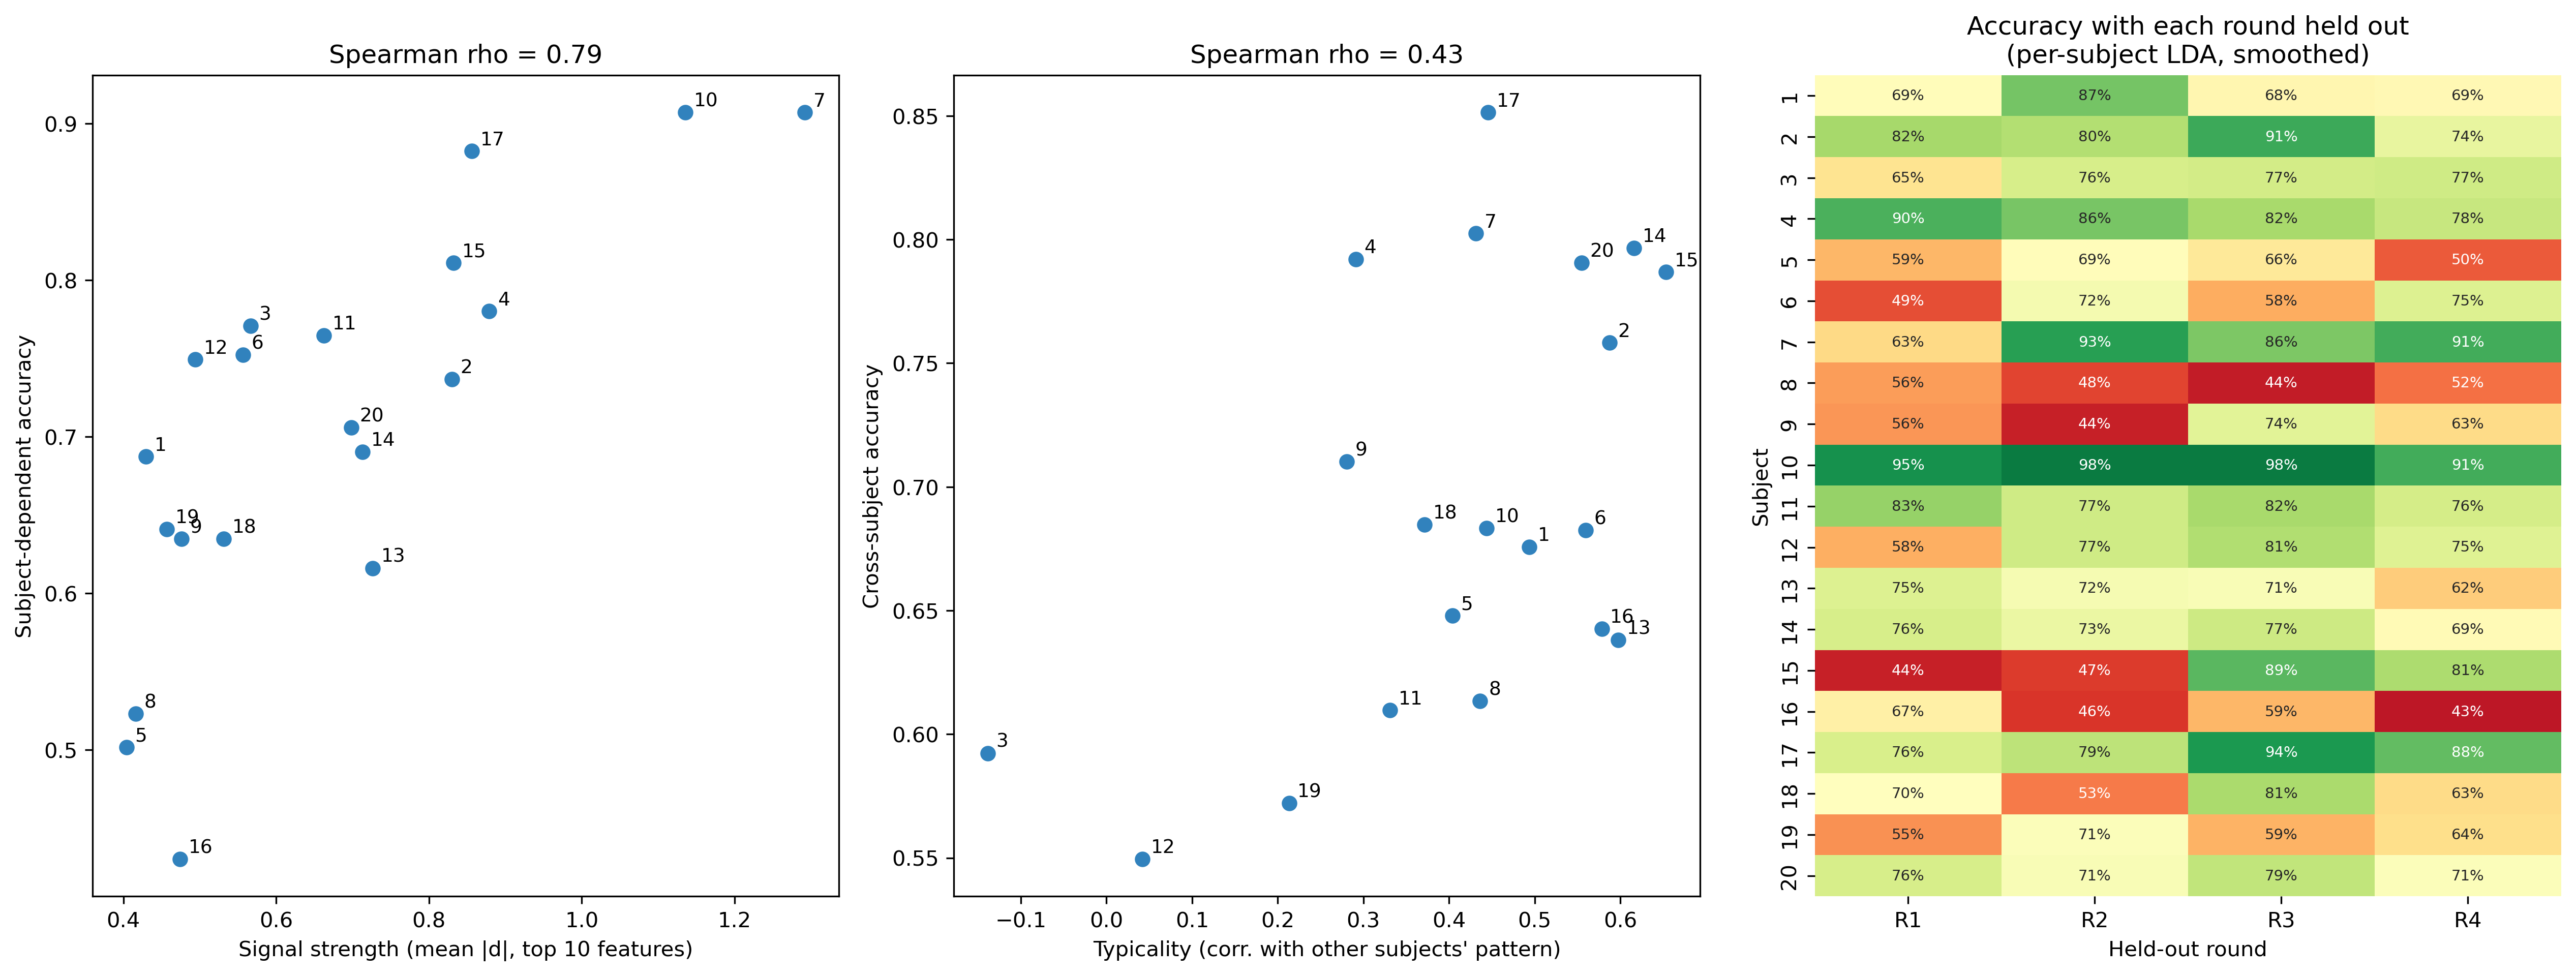
\includegraphics[width=\textwidth]{results/figures/subject_diagnostics.png}
    \caption{Per-subject diagnostics. Left: signal strength vs.\ subject-dependent accuracy. Middle: typicality vs.\ cross-subject accuracy. Right: accuracy of the per-subject pipeline when each round is held out (trained on the other three).}
    \label{fig:diagnostics}
\end{figure}

\subsection{Electrode placement and eye movements}
\label{sec:channels}

The NeuroPawn positions are fixed by the headset, but the MEMA recordings contain all 32 channels, so \texttt{channel\_selection.py} asks two questions: would another 8 EEG electrodes work better, and how much can the eye-movement channels alone tell apart the two states? The 29 EEG electrodes are candidates; the CPz reference and the two EOG channels are not.

\textbf{Protocol.} Greedy forward selection starts with no electrodes and repeatedly adds the one that most improves the score, up to 16. The score is the mean of the subject-dependent CV (per-subject LDA, leave-one-round-out) and cross-subject CV (LDA, GroupKFold by subject), computed on rounds 1--3 only. Each electrode set is then tested on round 4, which the search never saw, with fixed models: per-subject LDA trained on rounds 1--3 for the subject-dependent case, and a random forest trained on the other 19 subjects for the cross-subject case. These fixed models make the NeuroPawn numbers in Table~\ref{tab:channels} slightly different from Table~\ref{tab:results}, but all sets are compared under the same protocol.

\begin{table}[H]
\centering
\caption{Electrode sets compared on rounds 1--3 CV (used for the search) and on the untouched round~4 (smoothed accuracy, mean over 20 subjects).}
\label{tab:channels}
\small
\begin{tabular}{lcccc}
\toprule
 & \multicolumn{2}{c}{CV, rounds 1--3} & \multicolumn{2}{c}{Test, round 4} \\
Electrode set & Dependent & Cross & Dependent & Cross \\
\midrule
NeuroPawn 8 (F3, Fz, F4, C3, C4, Pz, O1, O2) & 69.8\% & 64.5\% & 70.6\% & 71.7\% \\
Greedy best 8 (T6, FP2, T3, TP8, Cz, P3, Pz, F7) & 77.5\% & 76.4\% & \textbf{81.4\%} & 79.0\% \\
All 29 EEG electrodes & 74.6\% & 73.7\% & 78.7\% & \textbf{79.3\%} \\
Mislabelled 8 (Fz, F3, F4, Cz, C4, P3, T6, O1) & 72.2\% & 69.8\% & 77.2\% & 75.2\% \\
EOG only (HEOL, HEOR) & 67.5\% & 65.5\% & 66.0\% & 63.3\% \\
\bottomrule
\end{tabular}
\end{table}

\begin{figure}[H]
    \centering
    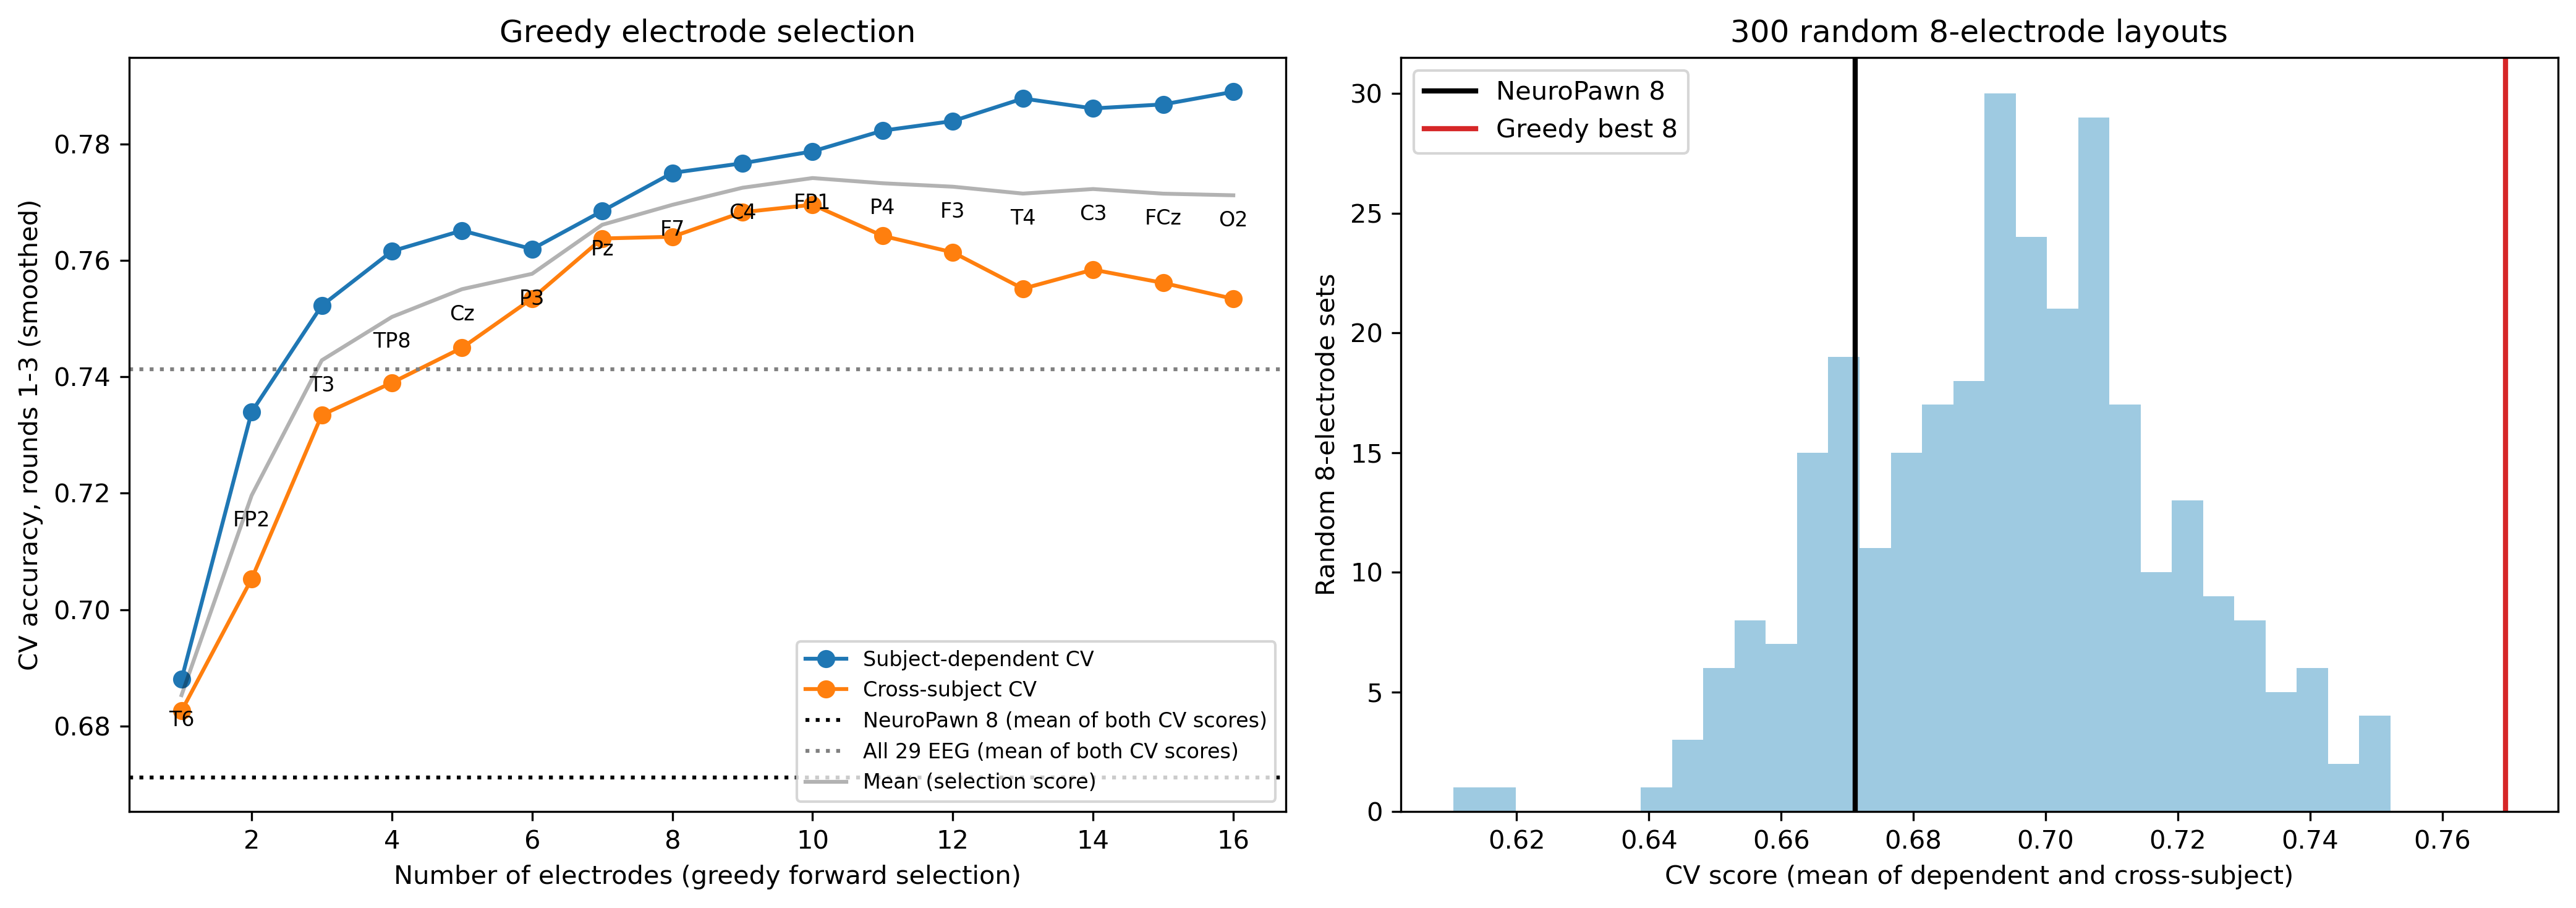
\includegraphics[width=\textwidth]{results/figures/channel_selection.png}
    \caption{Left: CV accuracy as greedy selection adds electrodes (labels show the electrode added at each step). Right: CV score of 300 random 8-electrode layouts. The greedy set was optimized on this same score, so its position is optimistic; round~4 in Table~\ref{tab:channels} is the fair comparison.}
    \label{fig:channels}
\end{figure}

\begin{itemize}
    \item \textbf{The NeuroPawn layout is a weak choice for this task.} It ranks at the 19th percentile of 300 random 8-electrode layouts. On round~4 the greedy set beats it by 10.7 points for calibrated users (better for 17 of 20 subjects; Wilcoxon $p = 0.002$) and 7.3 points for new users (15 of 20; $p = 0.009$).
    \item \textbf{Which electrodes.} The greedy set favours the sides of the head (T3, T6, TP8), adds the front (FP2 above the right eye, F7 at the left temple), and keeps three central-parietal sites (Cz, Pz, P3). The NeuroPawn layout has no temporal or frontopolar electrodes at all.
    \item \textbf{Eye movements carry part of the signal.} The two horizontal EOG channels alone reach 66\% and 63\% on round~4, well above the 55\% and 52\% baselines, so the participants' eyes moved differently during the attentive task. The electrodes the search prefers (temporal sites, FP2, F7) are also the ones that pick up most eye-movement and jaw/scalp-muscle activity. Part of the gain from a better layout is therefore likely to come from eye and muscle activity rather than brain activity. For a product this may still be a useful signal, but it is not evidence of a brain-based attention marker.
    \item \textbf{More is not always better.} All 29 electrodes (319 features) match the best 8 across subjects but are worse for calibrated users: with about 1{,}000 training windows per person, extra features mostly add noise. The CV curve flattens after about 8--10 electrodes.
\end{itemize}

\subsection{Comparison with the dataset paper}

The MEMA paper (Liu et al., Table~II) reports baselines for the same data and splits (rounds 1--3 vs.\ round~4, and leave-one-subject-out), but it classifies all \emph{three} states (attentive, neutral, relaxed) with all 32 channels. To compare like with like, \texttt{paper\_comparison.py} runs this project's pipeline on the 3-class task, reusing the models selected above without new tuning.

\begin{table}[H]
\centering
\caption{3-class attention classification: accuracy and macro F1 (\%), mean over 20 subjects. This project: 4~s windows, raw / 5~s smoothed. The paper's window length, features and averaging are not stated, so the comparison is approximate.}
\label{tab:paper}
\small
\begin{tabular}{lcccc}
\toprule
 & \multicolumn{2}{c}{Subject-dependent} & \multicolumn{2}{c}{Cross-subject} \\
Method & Accuracy & F1 & Accuracy & F1 \\
\midrule
Paper, best classical (DT / SVM) & 82.4 & 57.8 & 62.3 & 43.4 \\
Paper, best overall (EEGNet) & 85.1 & 59.6 & 64.8 & 45.1 \\
Paper, range of 6 methods & 78.7--85.1 & 47.6--59.6 & 56.0--64.8 & 41.9--45.2 \\
\midrule
This project, all 29 EEG electrodes & 66.9 / 70.4 & 60.3 / 63.3 & 63.4 / 69.1 & 54.5 / 59.3 \\
This project, NeuroPawn 8 & 59.5 / 62.1 & 52.6 / 55.1 & 54.5 / 59.4 & 46.6 / 50.3 \\
\bottomrule
\end{tabular}
\end{table}

Across subjects, this pipeline with 29 electrodes comes within 1.5 points of the paper's best accuracy on raw windows (63.4\% vs.\ 64.8\%) and exceeds it after smoothing (69.1\%). Its macro F1 is 9--14 points higher than any of the paper's methods. Within subjects, the paper's accuracy is much higher (79--85\% vs.\ 67--70\%), but its F1 is lower than or equal to this pipeline's (48--60\% vs.\ 60--63\%). High accuracy with low macro F1 usually means a classifier is mostly predicting the two long states and missing the short neutral state (one minute per round), which this pipeline handles better through balanced class weights. With only the NeuroPawn electrodes, the 3-class task is clearly harder (about 60\% accuracy).

\subsection{Key Observations}

\begin{enumerate}
    \item \textbf{Where the electrodes are matters as much as the model.} Moving the same 8-electrode budget to better positions gained 7--11 points, more than any modelling change.
    \item \textbf{Per-subject normalization matters most across people.} In an earlier experiment (on the mislabelled electrode set), per-subject z-scoring alone moved cross-subject accuracy from 57.4\% to 61.8\%. It removes each person's overall amplitude and spectral offsets, which are larger than the differences between attention states.
    \item \textbf{Temporal context helps.} Longer windows (Table~\ref{tab:windows}) and probability smoothing both add context. Figure~\ref{fig:smoothing} shows that accuracy keeps rising with longer smoothing horizons. The 5~s setting was fixed in advance and is the one reported; the curve is only a sensitivity analysis, and choosing the horizon from it would be tuning on the test set.
    \item \textbf{Model choice matters little once the inputs are normalized.} Linear models and tree ensembles are within about one point of each other in CV. For new users, a soft-voting ensemble of linear and tree models was chosen in 19 of 20 folds, but its CV advantage was small (0.4 points). For calibrated users, a shrinkage LDA was best: with only about 1{,}000 training windows per person, a strongly regularized linear model is hard to beat.
    \item \textbf{Feature selection did not help.} Keeping all 88 features was chosen in both scenarios.
    \item \textbf{Things that did not help.} Earlier experiments (on the mislabelled electrode set) found no gain from relative band power, Hjorth parameters, alpha asymmetry, z-scoring round~4 with its own statistics, or log-Euclidean covariance features.
    \item \textbf{Skepticism of literature benchmarks.} Some studies report 91.7\% (Aci et al., 2019) or 99.6\% (Wang \& Kim) on similar tasks. A common cause of such numbers is splitting overlapping windows from the same recording into training and test sets, which this project avoids by always holding out whole rounds or subjects. The dataset's own paper, which also holds out whole rounds and subjects, reports numbers in the same range as this project.
\end{enumerate}

\begin{figure}[H]
    \centering
    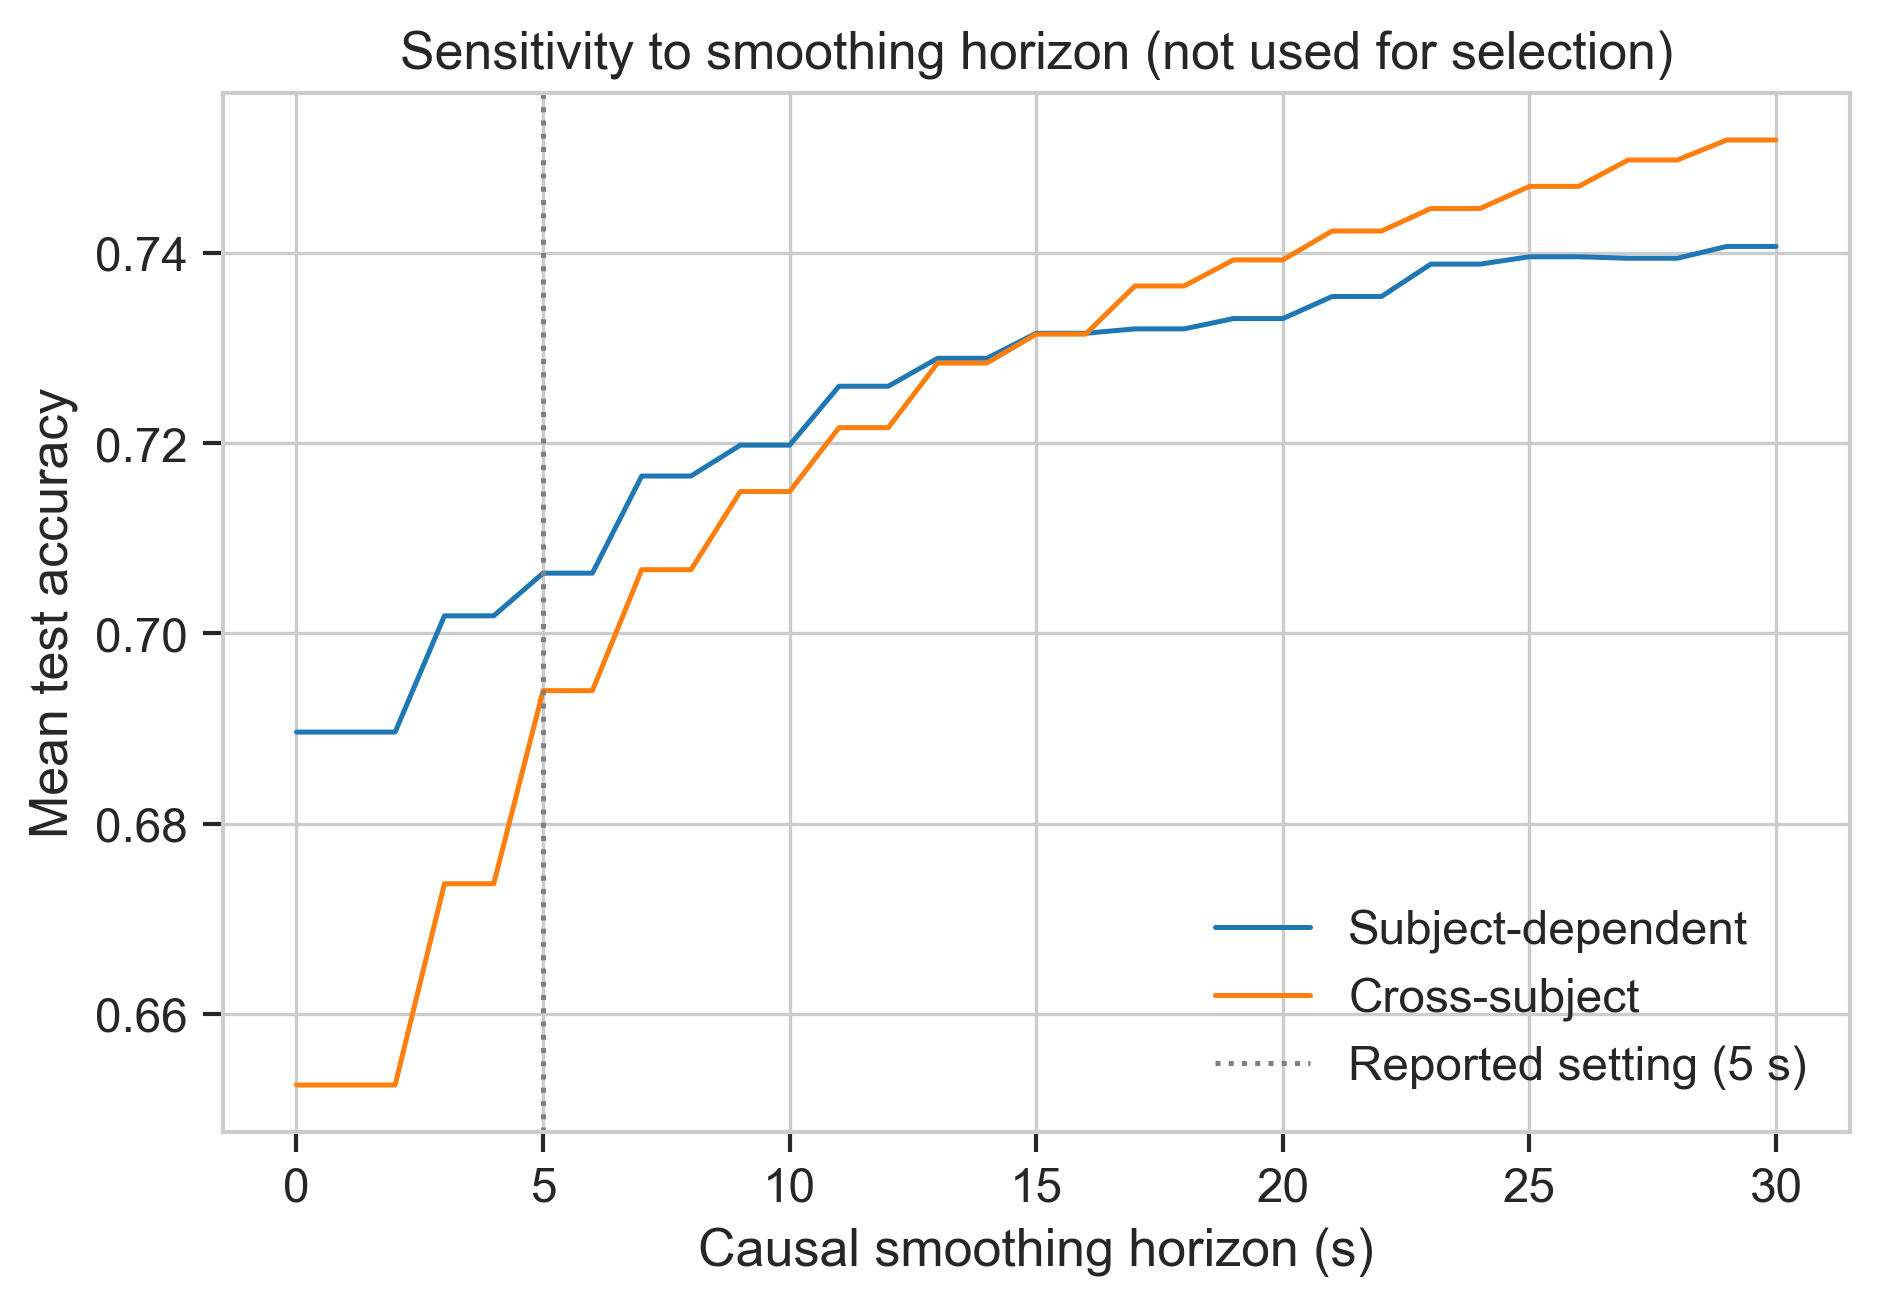
\includegraphics[width=0.7\textwidth]{results/figures/smoothing_curve.png}
    \caption{Mean test accuracy versus causal smoothing horizon (sensitivity analysis only; all reported numbers use the pre-set 5~s).}
    \label{fig:smoothing}
\end{figure}

\section{Limitations and Future Work}

Several limitations should be noted.

\begin{itemize}
    \item \textbf{Eye movements.} The EOG channels alone separate the states well above chance, so part of what any EEG model learns here may be eye behaviour during the task rather than attention itself. This is most likely for electrodes near the eyes and temples. Removing eye artifacts (for example by regressing out the EOG channels, or with ICA) before classification would show how much of the accuracy remains.
    \item \textbf{Block design favours smoothing.} Each trial is one to five minutes of a single state, so averaging over the past few seconds almost always averages over the same label. When attention switches quickly in real use, smoothing will help less, and every switch will be detected with a delay of up to the smoothing horizon plus the 4~s window.
    \item \textbf{Calibration data for normalization.} The cross-subject result assumes that a new user's feature statistics are known. Here they come from all of the held-out subject's recordings, which mix focused and unfocused time in roughly the same proportion as the other subjects. A deployed system would have to estimate them from a short unlabeled recording, and a very different mix of states in that recording would shift the statistics.
    \item \textbf{Shared design decisions.} The window length was chosen by cross-validation on rounds 1--3 of all subjects. Round~4 was never used, so the subject-dependent results are clean, but in the cross-subject evaluation the held-out subjects' rounds 1--3 contributed to this choice. Model, feature-selection method and hyperparameters were chosen fully inside the nested loop.
    \item \textbf{Offline filtering.} The band-pass filter is zero-phase (\texttt{sosfiltfilt}) over whole trials, which uses future samples. A real-time system would need a causal filter, which may change the results slightly.
    \item \textbf{Research-grade data.} The data was recorded with research-grade wet electrodes. A real NeuroPawn headset would add noise from dry electrodes and motion. Validating on actual consumer hardware is a necessary next step.
\end{itemize}

Future work: remove eye artifacts using the EOG channels and re-measure, test the alternative electrode layout on real hardware, add a short labelled calibration step for new users, and try deep learning architectures such as EEGNet, which learn spatial and temporal filters directly from the raw signal.

\section{Conclusion}

This project built an end-to-end pipeline from 90~GB of raw EEG text files to trained classifiers, simulating the constraints of a budget 8-channel, 125~Hz headset. With the headset's electrode positions, per-subject feature normalization, 4~s windows, model selection by grouped cross-validation, and 5~s causal smoothing, classical methods reach 70.6\% accuracy for a calibrated user and 69.4\% for an unseen user, against baselines of 55.1\% and 52.4\%. On the dataset's 3-class task with all electrodes, the same pipeline matches or beats the dataset authors' published baselines across subjects. The biggest single factor was electrode placement: the NeuroPawn layout is below the median of random 8-electrode layouts, and a better layout gained 7--11 points. Part of that gain, and part of the signal in general, appears to come from eye movements rather than brain activity, which should be checked before building on it. For NeuraXtension this means: per-subject normalization and a short calibration recording are worth having, and if the headset allows electrodes to be moved, temporal and parietal positions are worth testing.

\newpage
\section*{Project Experience Summary}

\textbf{EEG Attention State Classifier: Brain-Computer Interface}
\begin{itemize}
    \item Built an end-to-end Python pipeline (NumPy, SciPy, scikit-learn, LightGBM) that turns 90~GB of raw 32-channel EEG into an 8-channel, 125~Hz attention classifier matching a budget consumer headset.
    \item Reached 70.6\% accuracy for calibrated users and 69.4\% for unseen users (baselines 55.1\% and 52.4\%), using per-subject feature normalization, tuned window length, model ensembling and causal probability smoothing; on the dataset's 3-class task, matched or exceeded the dataset authors' published cross-subject baselines.
    \item Selected models without test-set leakage using grouped and nested cross-validation (leave-one-round-out and leave-one-subject-out), comparing 55 pipeline configurations (5 feature-selection methods $\times$ 11 classifier settings and ensembles) for each of 20 held-out subjects.
    \item Ran a greedy electrode-selection study over 29 EEG channels, finding an 8-electrode layout that improved held-out accuracy by 7--11 percentage points over the headset's fixed layout, and used the EOG channels to show that eye movements carry part of the signal.
    \item Parallelized the nested evaluation with joblib across 16 CPU threads, completing the full cross-subject model search in about 25 minutes.
\end{itemize}

\end{document}
